\documentclass[12pt,fleqn]{article}\usepackage{../common}
\begin{document}
Yaklasiksal SVD ile Tavsiye Sistemleri

Gecmis verilere bakarak bir kullanicinin hic seyretmedigi bir filme nasil
not verecegini tahmin etmek unlu Netflix yarismasinin konusuydu. Onceki bir
yazi {\em SVD, Toplu Tavsiye}'de benzer bir veri seti Movielens uzerinde
SVD uygulayarak once boyut azaltmistik, azaltilmis boyut uzerinden yeni (o
film icin notu bilinmeyen) bir kullanicinin diger mevcut kullanicilara
mesafesini hesaplamis, ve boylece begeni acisindan en cok benzedigi diger
kullaniciyi bulmustuk (birkac tane de bulunabilir). Bu kullanicinin bir
film icin verdigi notu yeni kullanici icin tahmin olarak baz almistik.

SVD uygulamanin tek yontemi bu degil. Netflix yarismasinda kullanilan [1]
bir yaklasim soyle; alttaki SVD ayristirmasina bakalim,

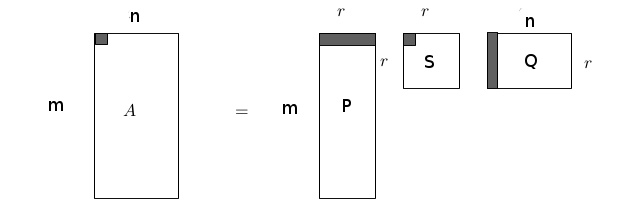
\includegraphics[height=4cm]{svdapprox_1.png}

1. kullanicini 1. filme verdigi not ustte koyu gosterilen satirlarin
carpimi ile oluyor, eger ufak harfler ve kullanici (user) icin $u$, film
icin $i$ indisini kullanirsak, ve $q,p$ vektorlerini $Q,P$ matrislerinin
sirasiyla kolon ve satirlarini gostermek icin kullanirsak, ayristirma
sonrasi begeni degeri (onemli bir kismi daha dogrusu) $q_i^Tp_u$
carpimindadir. Carpim icinde $S$'ten gelecek tekil degeri (singular value)
ne olacak?  Simdi formulasyonu biraz degistirelim, bu degeri carpim disina
alarak birkac toplam olarak gosterebiliriz. Bu toplamlar mesela bir
kullanicinin ne kadar yanli (bias) not verdigini, ya da bir filmin kabaca,
ortalama nasil not almaya meyilli oldugunu modelleyebilirler (ki bu da bir
yanlilik olcusu). Ayrica tum filmlere verilen notlarin yanliligi da
olculebilir. Tum bunlari bir araya koyarsak, bir begeni notunu tahmin
edecek formul soyle gosterilebilir,

$$
\hat{r}_{ui} = \mu + b_i + b_u + q_i^Tp_u
$$

$\mu$ bir skalar, tum filmlere verilen ortalamayi gosteriyor, ki tum
begenilerin sayisal ortalamasi uzerinden basit bir sekilde hizla
hesaplanabilir. $\hat{r}_{ui}$'ya bir tahmin dedik cunku modelimizdeki
vektorlerin degerlerini bulduktan sonra (egitim verisiyle bu hesabi
yapacagiz) modeli kullanarak gercek not $r_{ui}$ icin bir
tahmin yapmaya ugrasacagiz.

Egitim icin ne yapmali? Minimize edecegimiz bir hedef fonksiyonu kuralim,
ki cogunlukla bu karesi alinmis hata ile olur. Mesela gercek not
$r_{ui}$ degerinden tahmin notu $\hat{r}_{ui}$'yi cikartip karesini
alabiliriz. Bu islemi tum $u,i$'ler icin yaparak sonuclari toplariz, ve bu
toplami minimize etmeye ugrasabiliriz. Yani


$$
\min_{b*,q*,p*} \sum_{u,i} (r_{ui} - \hat{r}_{ui})^2 + 
\lambda (b_i^2 + b_u^2 + ||q_i||^2 + ||p_u||^2)
$$

$$
= \min_{b*,q*,p*} \sum_{u,i} (r_{ui} - \mu - b_i - b_u - q_i^Tp_u)^2 + 
\lambda (b_i^2 + b_u^2 + ||q_i||^2 + ||p_u||^2)
$$

Kisaltma olarak $e_{ui}$ tanimlayalim, bu faydali olabilir, formuldeki ilk
parantez icindeki kisimda $e_{ui}$ kullanmak uzere,
$$ e_{ui} := r_{ui} - \hat{r}_{ui} $$

$\lambda$ ile carpilan bolum regularizasyon icin. Istatistik, yapay
ogrenim, optimizasyon alanlarinda modelimizin asiri uygunluk (overfitting)
yapmasini engellemek icin regularizasyon kullanilir, bunun icin istedigimiz
degiskenlerin fazla buyumesini cezalandiririz, ustteki minimizasyon
modelinde bu ceza icin tum degerlerin buyuklugunu (magnitude) hesapladik
-skalar degerlerin karesini, vektor degerlerinin kare norm'unu alarak- ve
bu buyuklukleri bizim disaridan set edebilecegimiz bir sabitle carpilmasi
uzerinden minimizasyon problemine direk dahil ettik. Boylece bu buyuklukler
formulasyona dahil oldular ve azaltilma hedefinin bir parcasi haline
geldiler. Yani hem $e_{ui}^2$ hem de hatayi olusturan degerlerin kendileri
minimize edilecek.

Rasgele Gradyan Inisi (Stochastic Gradient Descent -SGD-)




$$
b_u \leftarrow b_u + \gamma (e_{ui} - \lambda \cdot b_u)
$$

$$
b_i \leftarrow b_i + \gamma (e_{ui} - \lambda \cdot b_i)
$$

$$
q_i \leftarrow q_i + \gamma (e_{ui}\cdot p_u - \lambda \cdot q_i)
$$

$$
p_u \leftarrow p_u + \gamma (e_{ui}\cdot q_i - \lambda \cdot p_u)
$$


\inputminted[fontsize=\footnotesize]{python}{ssvd.py}

\begin{minted}[fontsize=\footnotesize]{python}
import pandas as pd
import ssvd
d =  np.array(
[[  5.,   5.,   3.,  nan,   5.,   5.],
 [  5.,  nan,   4.,  nan,   4.,   4.],
 [ nan,   3.,  nan,   5.,   4.,   5.],
 [  5.,   4.,   3.,   3.,   5.,   5.],
 [  5.,   5.,  nan,  nan,  nan,   5.]
])
data = pd.DataFrame (d, columns=['0','1','2','3','4','5'],
       index=['Ben','Tom','John','Fred','Bob'])
mu,b_u,b_i,q_i,p_u = ssvd.ssvd(data,rank=3)
print mu
print 'b_u',b_u
print 'b_i',b_i
print 'q_i',q_i
print 'p_u',p_u
u = 4; i = 2
r_ui_hat = mu + b_i[i] + b_u[u] + np.dot(q_i[:,i].T,p_u[u,:])
print r_ui_hat
\end{minted}

\begin{verbatim}
rank 3
4.31388888889
b_u [ 0.05129388  0.01927226  0.0206893   0.0065487   0.06568321]
b_i [ 0.07820389  0.01958841 -0.03217881  0.01561187  0.04071886  0.07140383]
q_i [[ 0.03132989  0.02957741  0.02802317  0.02951804  0.0301854   0.03108419]
 [ 0.03132989  0.02957741  0.02802317  0.02951804  0.0301854   0.03108419]
 [ 0.03132989  0.02957741  0.02802317  0.02951804  0.0301854   0.03108419]]
p_u [[ 0.03053543  0.03053543  0.03053543]
 [ 0.0295772   0.0295772   0.0295772 ]
 [ 0.02963018  0.02963018  0.02963018]
 [ 0.02921864  0.02921864  0.02921864]
 [ 0.03100583  0.03100583  0.03100583]]
4.34999993855
\end{verbatim}


\begin{minted}[fontsize=\footnotesize]{python}
import pandas as pd, os
df = pd.read_csv("%s/Downloads/movielens.csv" % os.environ['HOME'] ,sep=';')
print df.shape
df = df.ix[:,1:3700] # id kolonunu atla,
df.columns = range(3699) # kolon degerlerini tekrar indisle
print df.shape
\end{minted}

\begin{verbatim}
(6040, 3731)
(6040, 3699)
\end{verbatim}

\begin{minted}[fontsize=\footnotesize]{python}
import ssvd
df_train, test_data = ssvd.create_training_test(df,rowlim=500,collim=300)
print len(test_data)
\end{minted}

\begin{verbatim}
501
\end{verbatim}


\begin{minted}[fontsize=\footnotesize]{python}
import ssvd
mu,b_u,b_i,q_i,p_u = ssvd.ssvd(df_train,rank=25)
print 'mu',mu
\end{minted}

\begin{verbatim}
rank 25
mu 3.23841096846
\end{verbatim}


\begin{minted}[fontsize=\footnotesize]{python}
rmse = 0; n = 0
for u,i,real in test_data:
    r_ui_hat = mu + b_i[i] + b_u[u] + np.dot(q_i[:,i].T,p_u[u,:])
    rmse += (real-r_ui_hat)**2
    n += 1
    #print u,i,real, r_ui_hat
print "rmse", np.sqrt(rmse / n)
\end{minted}

\begin{verbatim}
rmse 0.878340489577
\end{verbatim}










Kaynaklar

\url{http://sifter.org/~simon/journal/20061211.html}

Koren, Bell, {\em Recommender Systems Handbook},
\url{http://www.cs.bme.hu/nagyadat/Recommender_systems_handbook.pdf}

\url{http://www2.research.att.com/~volinsky/papers/ieeecomputer.pdf}

\url{http://www.cs.nyu.edu/~yann/talks/lecun-20071207-nonconvex.pdf}

\url{http://courses.cs.washington.edu/courses/cse528/09sp/sanger_pca_nn.pdf}

\url{http://users.ics.aalto.fi/oja/Oja1982.pdf}

\url{http://arxiv.org/pdf/1308.3509}

\url{http://www.maths.qmul.ac.uk/~wj/MTH5110/notes/MAS235_lecturenotes1.pdf}

\url{http://heim.ifi.uio.no/~tom/powerandqrslides.pdf}

\url{http://math.stackexchange.com/questions/649701/gradient-descent-on-non-convex-function-works-but-how}

\end{document}
